\chapter{REVISÃO DE LITERATURA}\label{chap:fundamentacaoTeorica}

Neste capítulo será incluso fundamentação teórica e citações da forma aqui apresentada neste exemplo.\cite{Ogata2010}

A Figura~\ref{fig:figura1}\ldots (incluir algumas figuras exemplo)\ldots

\begin{figure}[!htb]
    \centering
    \caption{Controle de temperatura de um forno elétrico}\label{fig:figura1}
    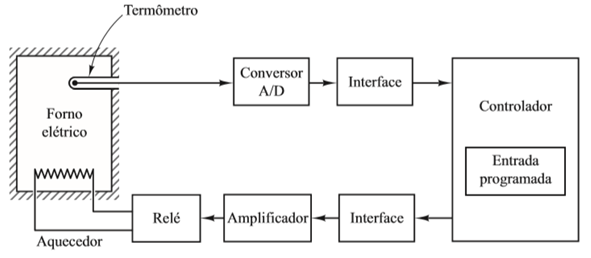
\includegraphics[width=0.7\textwidth]{figuras/figu1.png}
    \fonte{\citeonline{Ogata2010}}
\end{figure}
